\documentclass[aspectratio=169]{beamer}
\usepackage[utf8]{inputenc}
\usepackage[T1]{fontenc}
\usepackage{hyperref}
\usepackage{amsmath}
\usepackage{amssymb}
\usepackage{mathtools}
\usepackage{bbold}
\usepackage{booktabs}
\usepackage{minted}
\definecolor{LightGray}{gray}{0.95}
\usetheme{trex}

\usemintedstyle{manni}
%\usemintedstyle{colorful}
\setminted{baselinestretch=1.2,bgcolor=LightGray}

\newcommand{\tabitem}{\hspace{2ex}\llap{\scriptsize{$\blacksquare$}}\hspace{1ex}}

\author{François Coppens}
\institute{Université de Versailles Saint-Quentin-en-Yvelines}
\date{17/05/2021}
\title{A Mixed-precision exploration of CHAMP}

\begin{document}

  \maketitle
  
  \section{Quick reminders}
  
    \begin{frame}{Code prerequisites}
      \textbf{Language/compiler support}
      \begin{itemize}
        \item C/C++/\texttt{clang:} LLVM versions 4.0 -- 15.0
        \item Fortran/\texttt{flang:} LLVM versions $\leq7.0$
      \end{itemize}
      \textbf{SSH connection to OLYMPE}\\
      \texttt{> ssh -X <username>@olympe.calmip.univ-toulouse.fr}\\
      \textbf{Minimal environment}
      \begin{enumerate}
        \item \texttt{> export MODULEPATH=\$\{MODULEPATH\}:/usr/local/trex/modulefiles}
        \item \texttt{> module load verificarlo}
      \end{enumerate}
      \textbf{Verificarlo Singularity container}\\
      \texttt{> sing-verificarlo} 
    \end{frame}
    
    \begin{frame}{Supported languages}
      Verificarlo is a LLVM-based compiler extension. To this end Verificarlo offers compiler wrappers for the languages:\\
      
      \begin{itemize}
        \item[C] \texttt{verificarlo-c}
        \item[C++] \texttt{verificarlo-c++}
        \item[Fortran] \texttt{verificarlo-f}
      \end{itemize}
    \end{frame}
      
    \begin{frame}{Compiling and linking individual files}
      To compile and link a single source file\\
      \texttt{verificarlo-<lang> source-file.<lang> -o <executable name>}\\
      \vspace{1em}
      Or compile and link several files\\
      \texttt{verificarlo-<lang> -c source-file1.<lang> -o source-file1.o}\\
      \texttt{verificarlo-<lang> -c source-file2.<lang> -o source-file2.o}\\
      \texttt{...}\\
      \texttt{...}\\
      
      \texttt{verificarlo-<lang> source-file1.o source-file2.o ... -o <executable>}
    \end{frame}


    \begin{frame}{With a build tool}
      To use the Verificarlo compiler and linker in Makefile or CMake projects we recommend setting the environment variables \texttt{CC}, \texttt{CXX} and \texttt{FC} for respectively the C, C++ and Fortran compiler.      \vspace{1em}\\
      These are usually respected by GNU Make and Kitware CMake, unless explicitly overridden by by the user. To do this execute the following commands in the terminal
      \vspace{1em}
      \begin{itemize}
        \item \texttt{export CC=verificarlo-c}
        \item \texttt{export CXX=verificarlo-c++}
        \item \texttt{export FC=verificarlo-f}
      \end{itemize}

    \end{frame}

    \begin{frame}{Linking against OpenMPI}
      Use OpenMPI wrapper scripts to include OpenMPI headers and libraries. Make sure to point these wrappers to the appropriate Verificarlo compiler wrappers by exporting the following environment variables    \vspace{1em}\\
      \begin{tabular}{ll}
        \tabitem\texttt{export CC=mpicc} & \tabitem\texttt{export OMPI\_C=verificarlo-c} \\
        \tabitem\texttt{export CXX=mpic++} & \tabitem\texttt{export OMPI\_CXX=verificarlo-c++} \\
        \tabitem\texttt{export FC=mpifort} & \tabitem\texttt{export OMPI\_FC=verificarlo-f}
      \end{tabular}\vspace{1em}\\
      This will ensure the compiler wrappers are chained in the correct order.
    \end{frame}
      
    \begin{frame}{Enabling the Delta-Debug option in Verificarlo}
      To use the Delta-Debug feature in Verificarlo the extra flag \textbf{\texttt{--ddebug}} needs to be passed to the compiler directly or as \texttt{CFLAGS/CXXFLAGS/FCFLAGS}\vspace{1em}\\
      \texttt{verificarlo-\{c|c++|f\} --ddebug \textbackslash}\\
      \texttt{  -c source-file.<lang> \textbackslash}\\
      \texttt{  -o source-file.o}\vspace{1em}\\
      or as\vspace{1em}\\
      \texttt{CFLAGS/CXXFLAGS/FCFLAGS += --ddebug}
          
    \end{frame}
    
    \section{Mixed precision exploration in CHAMP using Delta-Debug}
    
      \begin{frame}{Source-code localisation}
        \begin{itemize}
            \item Delta-Debug in Verificarlo
                  \begin{itemize}
                      \item \structure{Configurations} are the sets of floating-point instructions.
                      \item A \structure{bug} is a numerical instability.
                  \end{itemize}
            \item Find unstable instructions for rounding / cancellations.
            \item Find instructions that can be run in lower precision.
        \end{itemize}
    
        \begin{table}[h]
          \centering
          \begin{tabular}{lcr}
                Step           & Instructions with MCA noise & Numerically Stable \\
                \midrule
                1              & 1 2 3 4 . . . .             & stable             \\
                2              & . . . . 5 6 7 8             & unstable           \\
                \midrule
                3              & . . . . 5 6 . .             & stable             \\
                4              & . . . . . . 7 8             & unstable           \\
                \midrule
                5              & . . . . . . 7 .             & unstable           \\
                Result (ddmin) & . . . . . . 7 .             &                    \\
          \end{tabular}
        \end{table}
      \end{frame}
    
  \section{Setting up the Delta-Debug helper scripts}
    
    \begin{frame}{Steps involved}
      \begin{enumerate}
        \item Chose an observable: in this case it's the \textbf{total energy} and \textbf{one of the forces}
        \item Prepare \textbf{\texttt{ddRun}}: script that runs the code and extracts the observable to monitor from the output
        \item Prepare \textbf{\texttt{ddCmp}}: script that sets the \textbf{precision threshold} from the reference value and returns:
          \begin{itemize}
            \item \textbf{\texttt{true}/\texttt{pass}}: if precision of  current value does \textbf{NOT EXCEED} maximum deviation
            \item \textbf{\texttt{false}/\texttt{fail}}: if precision of  current value \textbf{EXCEEDS} the maximum deviation 
          \end{itemize}
        \item Prepare a small \textbf{\texttt{Makefile}}: to automate setting Verificarlo \textbf{backend}, \textbf{precision}, \textbf{\# of ddebug runs} and \textbf{\texttt{vfc\_ddebug}} invocation
      \end{enumerate}
    \end{frame}

    \begin{frame}[fragile]{\textbf{Step 1 and 2: \texttt{ddRun}}}
      \begin{minted}{bash}
OUTDIR=$1

BIN=./vfcdd_champ
INP=input.inp

for i in $(seq 1 1)
do
  $BIN -i $INP -o /tmp/res.dat 2> ${OUTDIR}/ddrun.error
  awk '/total E/{print$4}' /tmp/res.dat > $OUTDIR/res$i.dat
  rm /tmp/res.dat
done
      \end{minted}
    \end{frame}
    
    \begin{frame}[fragile]{\textbf{Step 3: \texttt{ddCmp 1/3}}}
      \begin{minted}{python}
import sys
import glob
import os
import numpy as np
import math

PRECISION_THRESHOLD = 5 # number of DECIMAL digits
REFDIR  = sys.argv[1]
CURRDIR = sys.argv[2]
res = np.zeros(shape=0)
      \end{minted}
    \end{frame}

    \begin{frame}[fragile]{\textbf{Step 3: \texttt{ddCmp 2/3}}}
      \begin{minted}{python}
def read_output(DIR, RES):
    resList = glob.glob(os.path.join(DIR, 'res*.dat'))
    resList += glob.glob(os.path.join(REFDIR, 'res*.dat'))
    for resFile in resList:
        with open(resFile) as f:
            RES = np.append(RES, float(f.read()))
    return RES
      \end{minted}
    \end{frame}


    \begin{frame}[fragile]{\textbf{Step 3: \texttt{ddCmp 3/3}}}
      \begin{minted}{python}
res = read_output(CURRDIR, Res)

s = math.log2(abs((res[0]-res[1])/res[1]))/math.log2(10)
          # see next slide

with open("{}/res.stat".format(CURRDIR), 'w') as f:
    print(f"Stat. file loc = {CURRDIR}/res.stat")
    f.write("s = {}\n".format(s))

sys.exit(1 if s < PRECISION_THRESHOLD else 0)
      \end{minted}
    \end{frame}

    \begin{frame}{Number of significant digits}
      Precision in number of bits
      \begin{align*}
	     s_2 = -\log_2\left|\frac{x_\mathrm{VPREC} - x_\mathrm{IEEE}}{x_\mathrm{IEEE}}\right|
      \end{align*}
      Precision in number decimals
      \begin{align*}
	     s_{10} = \frac{s_2}{\log_2(10)}
      \end{align*}
      
    \end{frame}

    \begin{frame}[fragile]{\textbf{Step 4: \texttt{Makefile}}}
      \begin{minted}{make}
NRUNS=1
PRECISION=24
BACKEND="libinterflop_vprec.so --precision-binary64=${PRECISION}"

dd: vfcdd_champ
  rm -rvf dd.line/
  INTERFLOP_DD_NRUNS=${NRUNS} VFC_BACKENDS=${BACKEND} \
  vfc_ddebug ddRun_vp ddCmp_vp

dderrors: dd.line/rddmin-cmp/dd.line.exclude
  bash -c "vim -q <(./vfc_dderrors.py ./vmc $<)"
      \end{minted}
    \end{frame}
    
    \begin{frame}[fragile]{Run CHAMP with Delta-Debug}
    \textbf{After running \texttt{make dd} you should see output like}
      \begin{verbatim}
INTERFLOP_DD_NRUNS=1 VFC_BACKENDS="libinterflop_vprec.so \
   --precision-binary64=17" vfc_ddebug ddRun_vp ddCmp_vp
dd.line/8a391a01211abd91e3d54cfeca2897f4 --( run )-> FAIL(0)
dd.line/8a391a01211abd91e3d54cfeca2897f4 --(cache) -> FAIL
dd.line/525c227b98a0ae2e100829a4100dbcf4 --( run )-> FAIL(0)
dd.line/4ebd0a8a27fa25253644536b5ea1cbe8 --( run )-> FAIL(0)
dd.line/8a8069fe0ee2b665eab4c7034fba118d --( run )-> PASS(+1->1)
dd.line/b434b51d52907341f6f05a9e4128d8e1 --( run )-> FAIL(0)
dd.line/53769469e1628356f7b2aa219c9df18a --( run )-> FAIL(0)
dd.line/d2d274f8db7675ba550c01ce6979c32a --( run )-> PASS(+1->1)
dd.line/93e0258c4d272730e115c64951366207 --( run )-> FAIL(0)
dd.line/c7d60fc315f6b8e0ec55cb39c6a4edd1 --( run )-> PASS(+1->1)
dd.line/91384f0e34618621669fdd58e04583c3 --( run )-> FAIL(0)
ddmin0 (0x0000000000521ced: splfit_ at splfit.f:47):
      \end{verbatim}
    \end{frame}

    \begin{frame}[fragile ]{Contents of \textbf{\texttt{dd.line}} 1/2}
      \begin{verbatim}
drwxr-xr-x. coppens p22064 04bb7a6780419ee429cd806fe66cce66
drwxr-xr-x. coppens p22064 05928b62472d3723566e3b4d193bcb2c
drwxr-xr-x. coppens p22064 0598f288b121391b3cd8f9f2e948c8d2
drwxr-xr-x. coppens p22064 d914463b3d0055e77e0128b74ceb5291
lrwxrwxrwx. coppens p22064 ddmin0 -> 05928b62472d3723566e3b4d193bcb2c
lrwxrwxrwx. coppens p22064 ddmin1 -> d914463b3d0055e77e0128b74ceb5291
drwxr-xr-x. coppens p22064 dee78da1159ba7d45cfd5809f9799e22
drwxr-xr-x. coppens p22064 df02513b130ff37c200ebf49f7aa22a7
drwxr-xr-x. coppens p22064 fd5e7760f41617300b4e5b49b6a55843
drwxr-xr-x. coppens p22064 ff680b1e38e2818b5e9f67029f123644
lrwxrwxrwx. coppens p22064 rddmin-cmp -> df02513b130ff37c200ebf49f7aa22a7
drwxr-xr-x. coppens p22064 ref
      \end{verbatim}
    \end{frame}

    \begin{frame}[fragile ]{Contents of \textbf{\texttt{dd.line}} 2/2}
      \begin{verbatim}
ff680b1e38e2818b5e9f67029f123644        ref
|-- dd.line.exclude                     |-- checkRef.err
|-- dd.line.include                     |-- checkRef.out
`-- dd.run1                             |-- dd.err
    |-- dd.compare.err                  |-- dd.line
    |-- dd.compare.out                  |-- dd.line.%%p
    |-- dd.run.err                      |-- dd.out
    |-- ddrun.error                     |-- ddrun.error
    |-- dd.run.out                      |-- res1.dat
    |-- res1.dat                        `-- res.stat
    |-- res.stat
    `-- returnVal
      \end{verbatim}
    \end{frame}
    
    \begin{frame}{Minimal sets}
      When done, minimal set can be found in \texttt{\$PWD/dd.line/rddmin-cmp}. It contains the files
      \begin{itemize}
        \item \textbf{\texttt{dd.line.exclude}:} contains the functions/subroutines that break at the chosen precision. 
        \item \textbf{\texttt{dd.line.include}:} contains the functions/subroutines that can be changed to the lower precision without affecting the precision of the total energy
      \end{itemize}
    \end{frame}
      
    \begin{frame}{CHAMP results for \textbf{total energy}}
      \begin{table}[h]
\caption{CHAMP/VMC Butadiene CIPSI. Investigated precision on TOTAL ENERGY for all functions.}
\label{table:te}
\begin{tabular}{@{}ll@{}}
                  \\ \midrule
Function name                          & Required precision (VPREC) \\ \midrule
\texttt{splfit}                        & Double                              \\
\texttt{ALL OTHERS}                    & Single                         \\

\end{tabular}
\end{table}
\textbf{Conclusion}: When only interested in the energy we can run most of CHAMP at single precision, potentially gaining a significant speedup. 

    \end{frame}

    \begin{frame}{CHAMP results for \textbf{forces}}
      \centering
      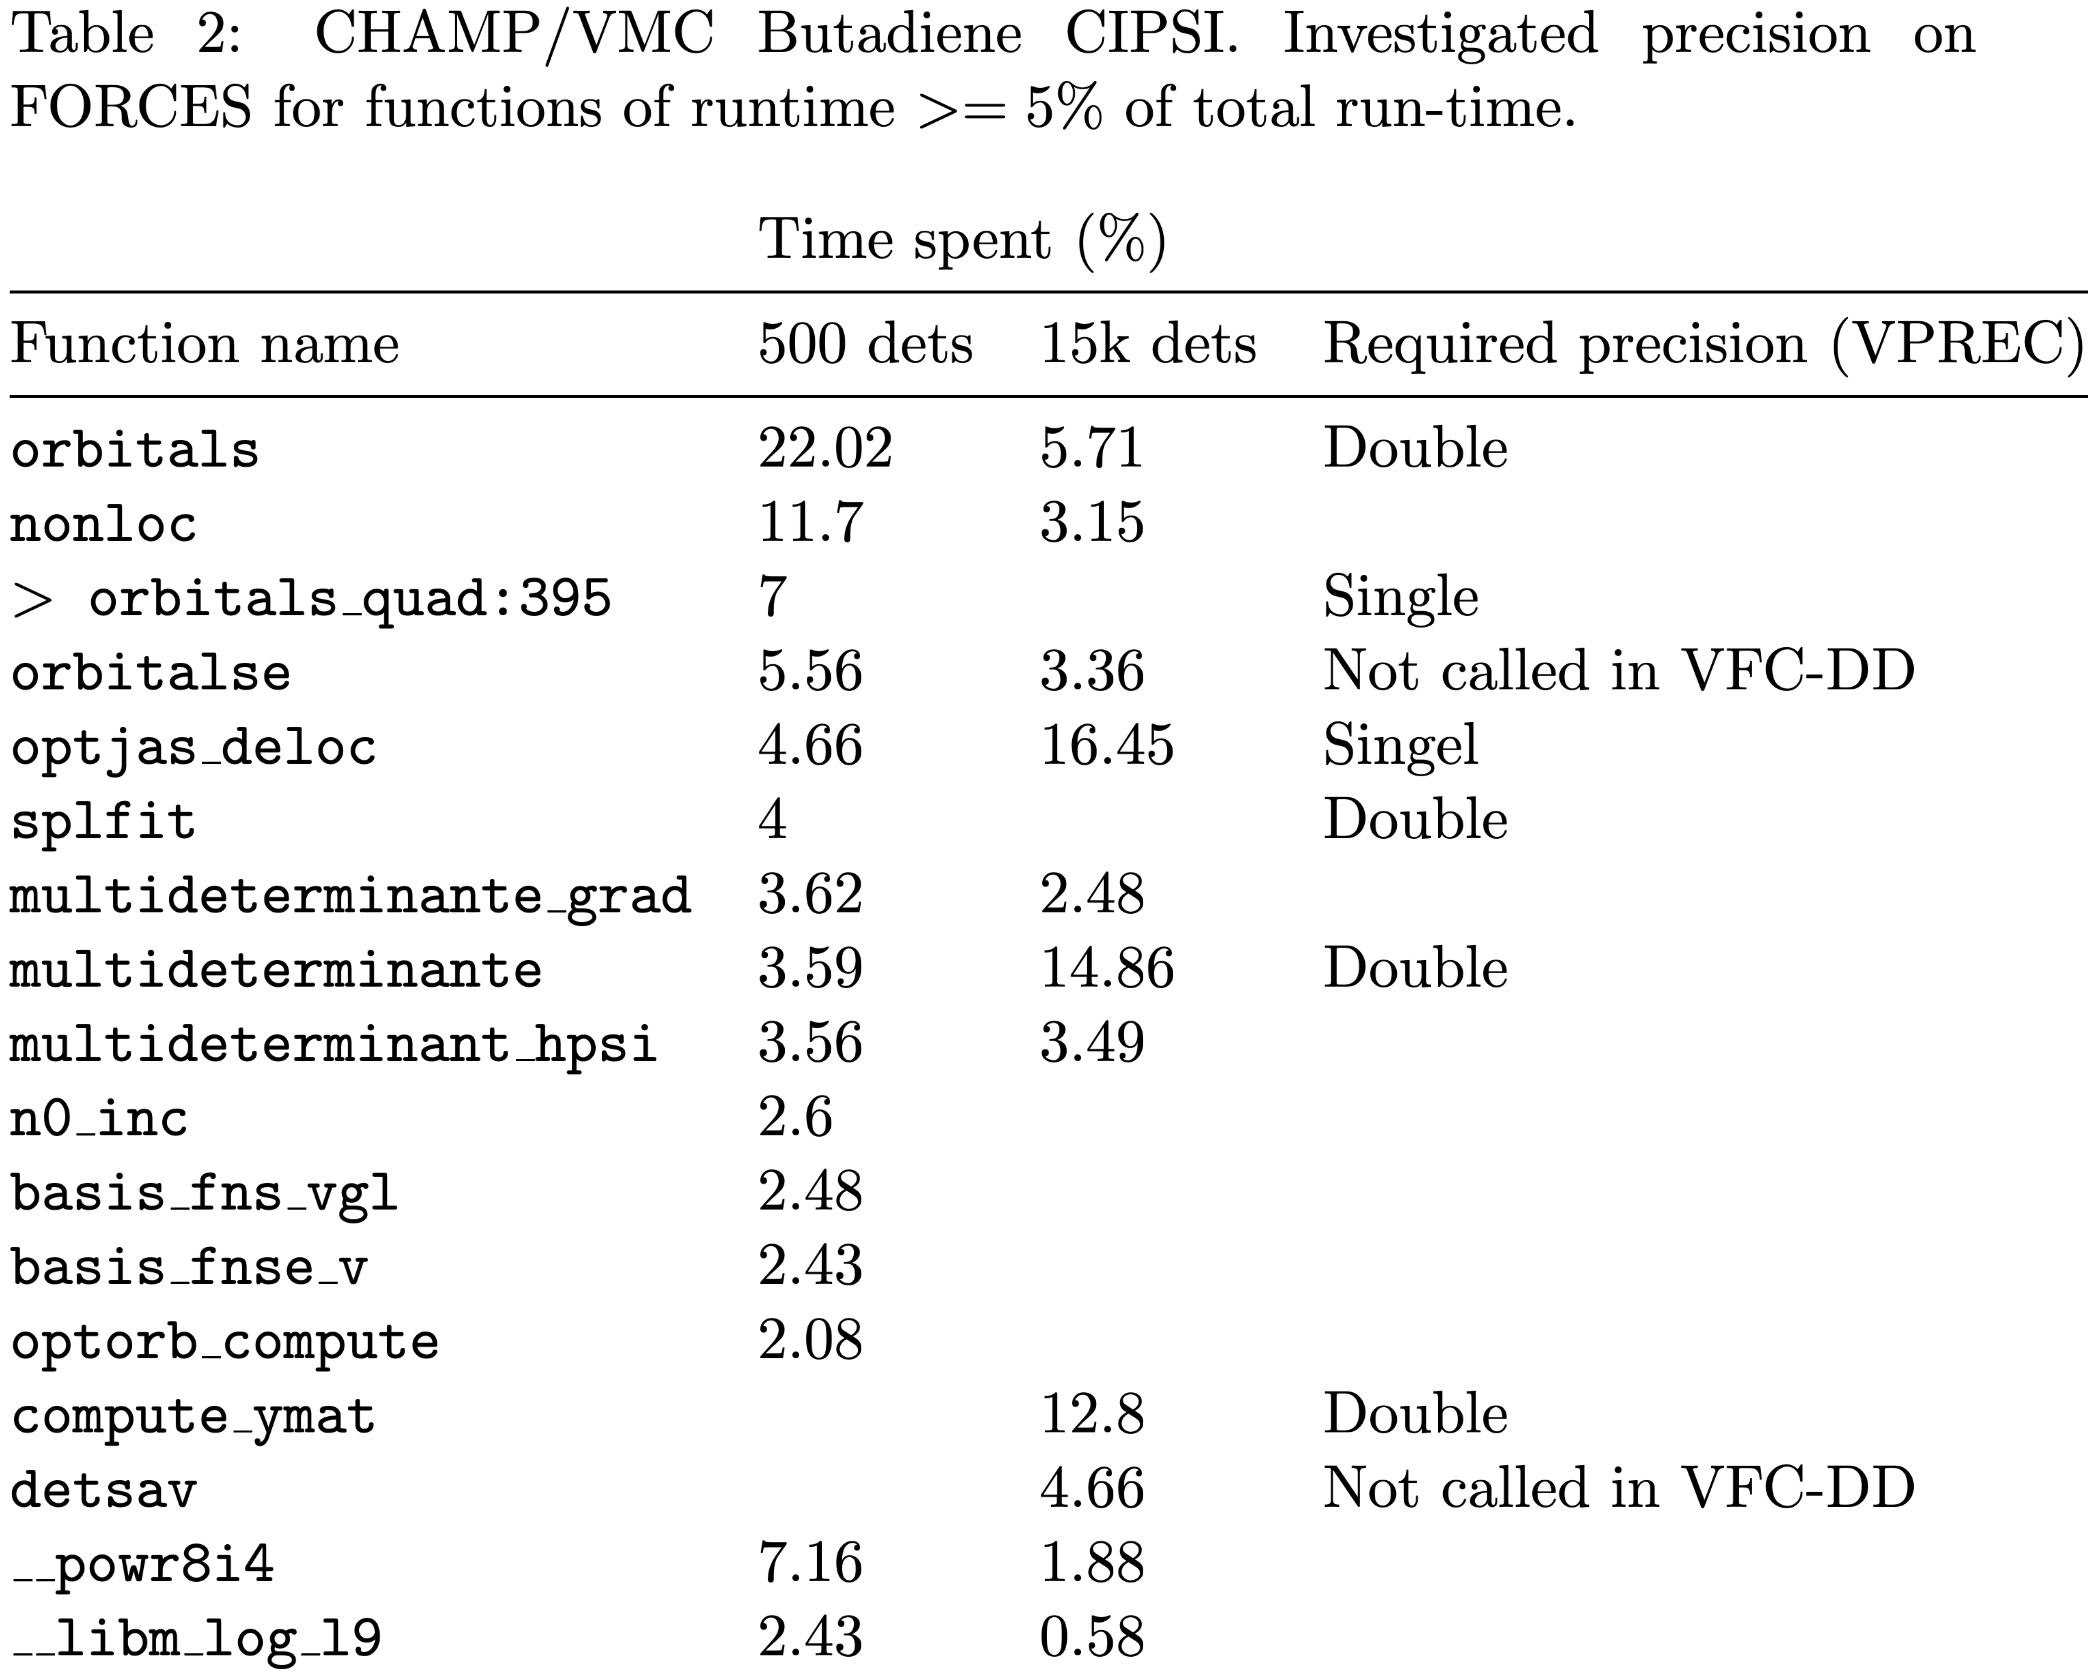
\includegraphics[width=0.5\linewidth]{forces.png}\\
      \textbf{Conclusion}: sometimes life is more complicated
    \end{frame}
    
    \begin{frame}{Pittfals compiling CHAMP with \texttt{flang-7}}
      \begin{itemize}
        \item[MPI] \texttt{flang-7} is not able to assign multiple file descriptors to the same file $\longrightarrow$ prevents from running more than one MPI process! 
      \end{itemize}
\textit{      MORE PROBLEMS TO BE ADDED}
    \end{frame}
  
\end{document}
